\documentclass[12pt]{article}
\usepackage{graphicx}
\usepackage{amsmath}
\usepackage{hyperref}
\usepackage{geometry}
\usepackage{enumitem}
\usepackage{float}
\usepackage{cite}
\usepackage{subfigure}
\usepackage[utf8]{inputenc}
\usepackage[T1]{fontenc}
\usepackage{booktabs}
\usepackage[table,xcdraw]{xcolor} % Enables gray colors for tables
\usepackage{multirow}
\usepackage{array}  
\usepackage{tabularx}
\usepackage{siunitx} 


\geometry{a4paper, margin=1in}

\setlength{\tabcolsep}{4pt} % Adjust column spacing
\renewcommand{\arraystretch}{2} % Increase row height spacing

\begin{document}

\title{Bipedal gait bio-mimicry using a foldable mechanism\\ \small Foldable Robotics Group Assignment 1}
\date{}
\author{Group 2: Jahnav Rokalaboina, Kunal Palasdeokar and Nihar Masurkar}

\maketitle

\section*{Project Outline }
Bipedalism is the ability of animals to walk or run by bearing weight on two legs, a trait often seen in birds and some mammals, including humans. Birds, such as ostriches, are a prime example of bipedal locomotion, using their strong limbs for walking and running at high speeds. This type of locomotion is characterized by distinct gait patterns, including walking, hopping, or running, which vary depending on terrain and speed. The skeletal structure of birds is adapted for efficient bipedal movement, with lightweight bones and muscular legs designed for propulsion. Despite variations in body size across bird species, their skeletal framework remains consistent, emphasizing flight and ground locomotion adaptation.

Types of gait in birds vary depending on their size, habitat and need for speed or stability. For example, ostriches, known for their remarkable running ability, use walking and sprinting gaits, with transitions to more complex patterns at higher speeds, such as bounding strides where both legs may leave the ground. These gait variations allow birds to efficiently adapt to their environment, balancing speed, endurance, and stability on different terrains. Researchers have also explored bipedal gait biomechanics to design bipedal robots. Bipedal robots that mimic bird locomotion leverage dynamic gait patterns and energy-efficient trajectories to achieve stability and agility on uneven terrain. This project focuses on studying and replicating such gait mechanics using a foldable mechanism. Utilizing the material's inherent stiffness and flexibility, the goal is to analyze the effects of gait transitions on speed and terrain adaptability, offering valuable insights for both robotics and biomechanical applications.

This project's scope is to replicate two legs of a bird, such as an ostrich, and study two primary gaits, walking and hopping, using a foldable five-bar mechanism. This mechanism’s kinematics are to be studied and simulated using MuJoCo (MuJoCo is a physics engine for detailed, efficient rigid body simulations); using servo motors and a microcontroller, the position and orientation of legs can be controlled to implement different gaits. The gait pattern can be created using the simulated mechanism and extracting the joint angles from the simulation to implement in the control of the robot; the simulated gait and experimental gait can be further compared and validated.



Using a five-bar linkage system leveraging the foldable mechanism, the biomimicry of an ostrich's legs mimics the intricate, multi-joint motions of real limbs, offering important insights into bipedal biomechanics. This design makes smoother and more flexible motion possible in robotic applications, which captures the kinematics and dynamics of different gaits. Biped biomechanism has been a hot research topic for decades thanks to its adaptability and low energy required to walk and get higher mobility. This project aims to study, develop, and mimic bipedal gait using foldable robotic techniques to further the utility and understanding of the nuances of foldable mechanisms’ structural rigidity and the flexibility of joints and links.

This project demands various skill sets, including but not limited to prototyping, simulation using MuJoCo, control theory, and designing the mechatronic system. Our team members have experience in the required skills for this project and hope to further our understanding of integrating complex systems using course material on foldable mechanisms, kinematics, and dynamics of five-bar mechanisms. Our ability to plan, execute, and validate this project throughout the semester takes into account our individual interests within the project and collective coordination to promptly meet the deliverables and deadlines.

A few of the deliverables of this course, foldable robotics, include kinematic and dynamic analysis of joints and links leveraging various foldable mechanisms that include spherical, hinge, prismatic joints, etc., and physics-based simulation using MuJoCo by defining all the joints and links. All of these concepts are being utilized and studied within this project's scope while studying a bipedal biomechanism for terrestrial locomotion. The foldable five-bar link mechanism is to be implemented as a leg of an ostrich, the size of which is chosen arbitrarily considering the torque capacity of servo motors and the weight of material used in making foldable joints and links.


%---------------------------------------------------------------------------------------------%

\subsection*{1. Background}

Compared to crawler or wheeled robots, bipedal robots have advantages when navigating rough terrains because of their discrete gait trajectories, giving them adaptability and mobility \cite{abourachid2016natural}. The anatomy of birds which rely on feet rather than wings for locomotion, like ostriches, over evolution, is adapted for agility and adaptability to different terrains, giving them different types of gaits. Ostriches have evolved with skeletal structures for running and stability. Their limbs play a critical role in balance and navigation, with muscles and joints working harmoniously to stabilize the body, particularly during directional changes or running at high speeds. Muscles such as digital flexors and extensors contribute significantly to propulsion, providing strength and flexibility during movement cycles \cite{rubenson2004gait}. Figure \ref{fig:ostritchanat} shows a dog's swing and stance phase during walking.


\begin{figure}[ht]
    \centering
    \subfigure[]{
        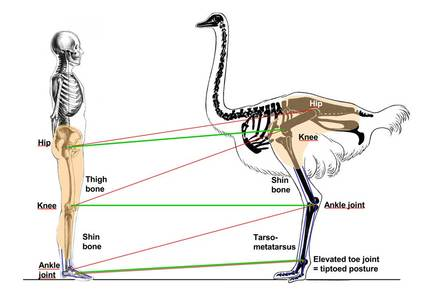
\includegraphics[width=0.4\textwidth]{figures/ostritch anatomy.jpg}
        \label{fig:ostritchanat}
    }
    \subfigure[]{
        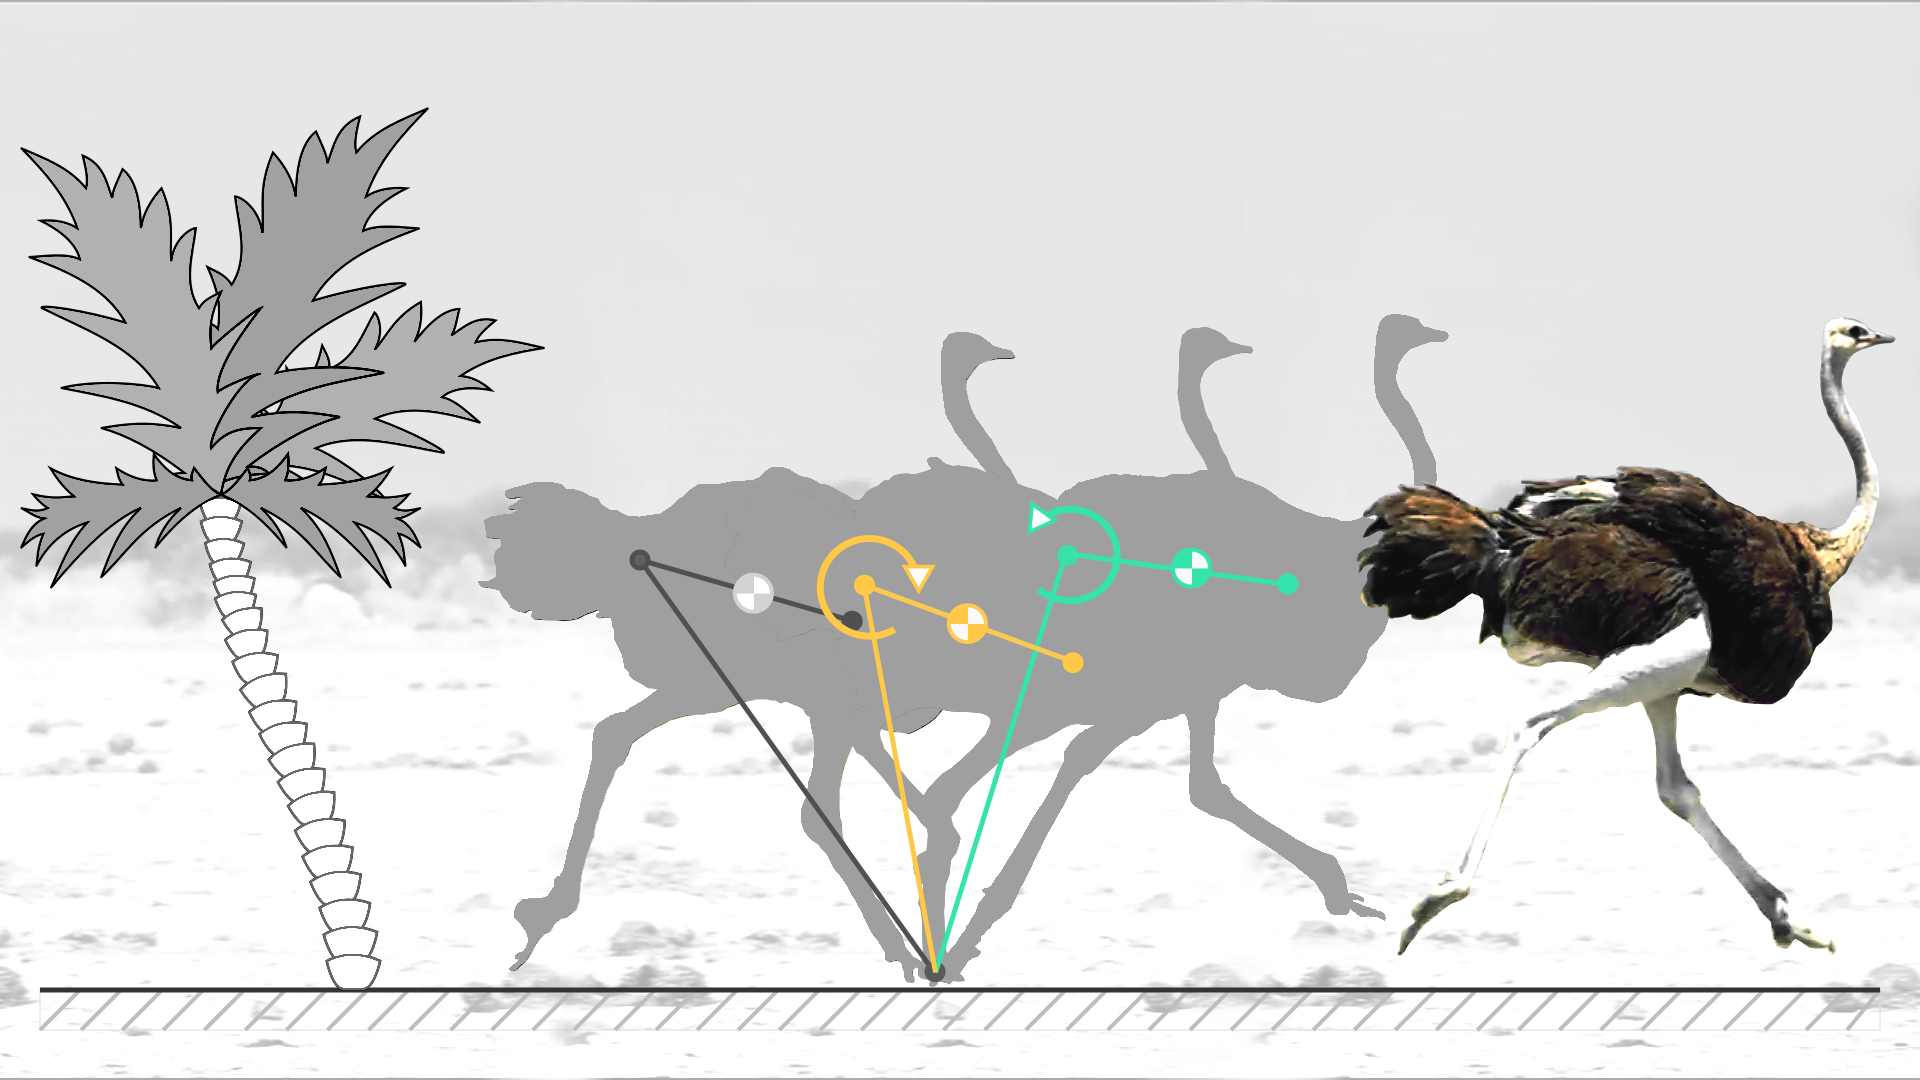
\includegraphics[width=0.5\textwidth]{figures/gaitostr.png}
        \label{fig:ostrgait}
    }
    \caption{Illustrations of bio-inspired bipedal mechanisms: (a) Comparative anatomy of human and ostrich bipedal walking structures; (b) Walking gait pattern of an ostrich.}
    \label{fig:combinedfigure}
\end{figure}

% \begin{figure*}[ht]
% \centering
% 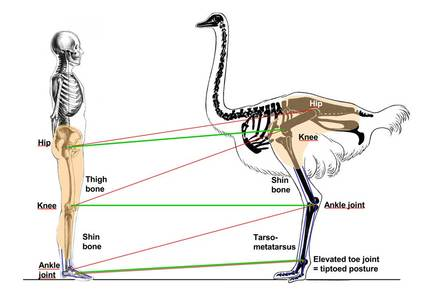
\includegraphics[scale=0.8]{figures/ostritch anatomy.jpg}
% \caption{Similarities in bipedal walking anatomy of human and an ostrich}
% \label{fig:ostritchanat}
% \end{figure*}

Ostriches exhibit a variety of gaits that adapt to different speeds and terrains. These gaits consist of walking, running, and hopping. Each gait involves a unique sequence of limb movements, impacting speed, posture, and stability. Figure \ref{fig:ostrgait} shows the walking gait of an ostrich. For example, in the running gait with moments of suspension—muscles stretch and contract eccentrically to store elastic energy, which enhances speed and reduces fatigue during sprinting \cite{drama2020b}. Understanding these natural gaits shows how ostriches can move efficiently and quickly irrespective of terrain topography.

% \begin{figure*}[ht]
% \centering
% 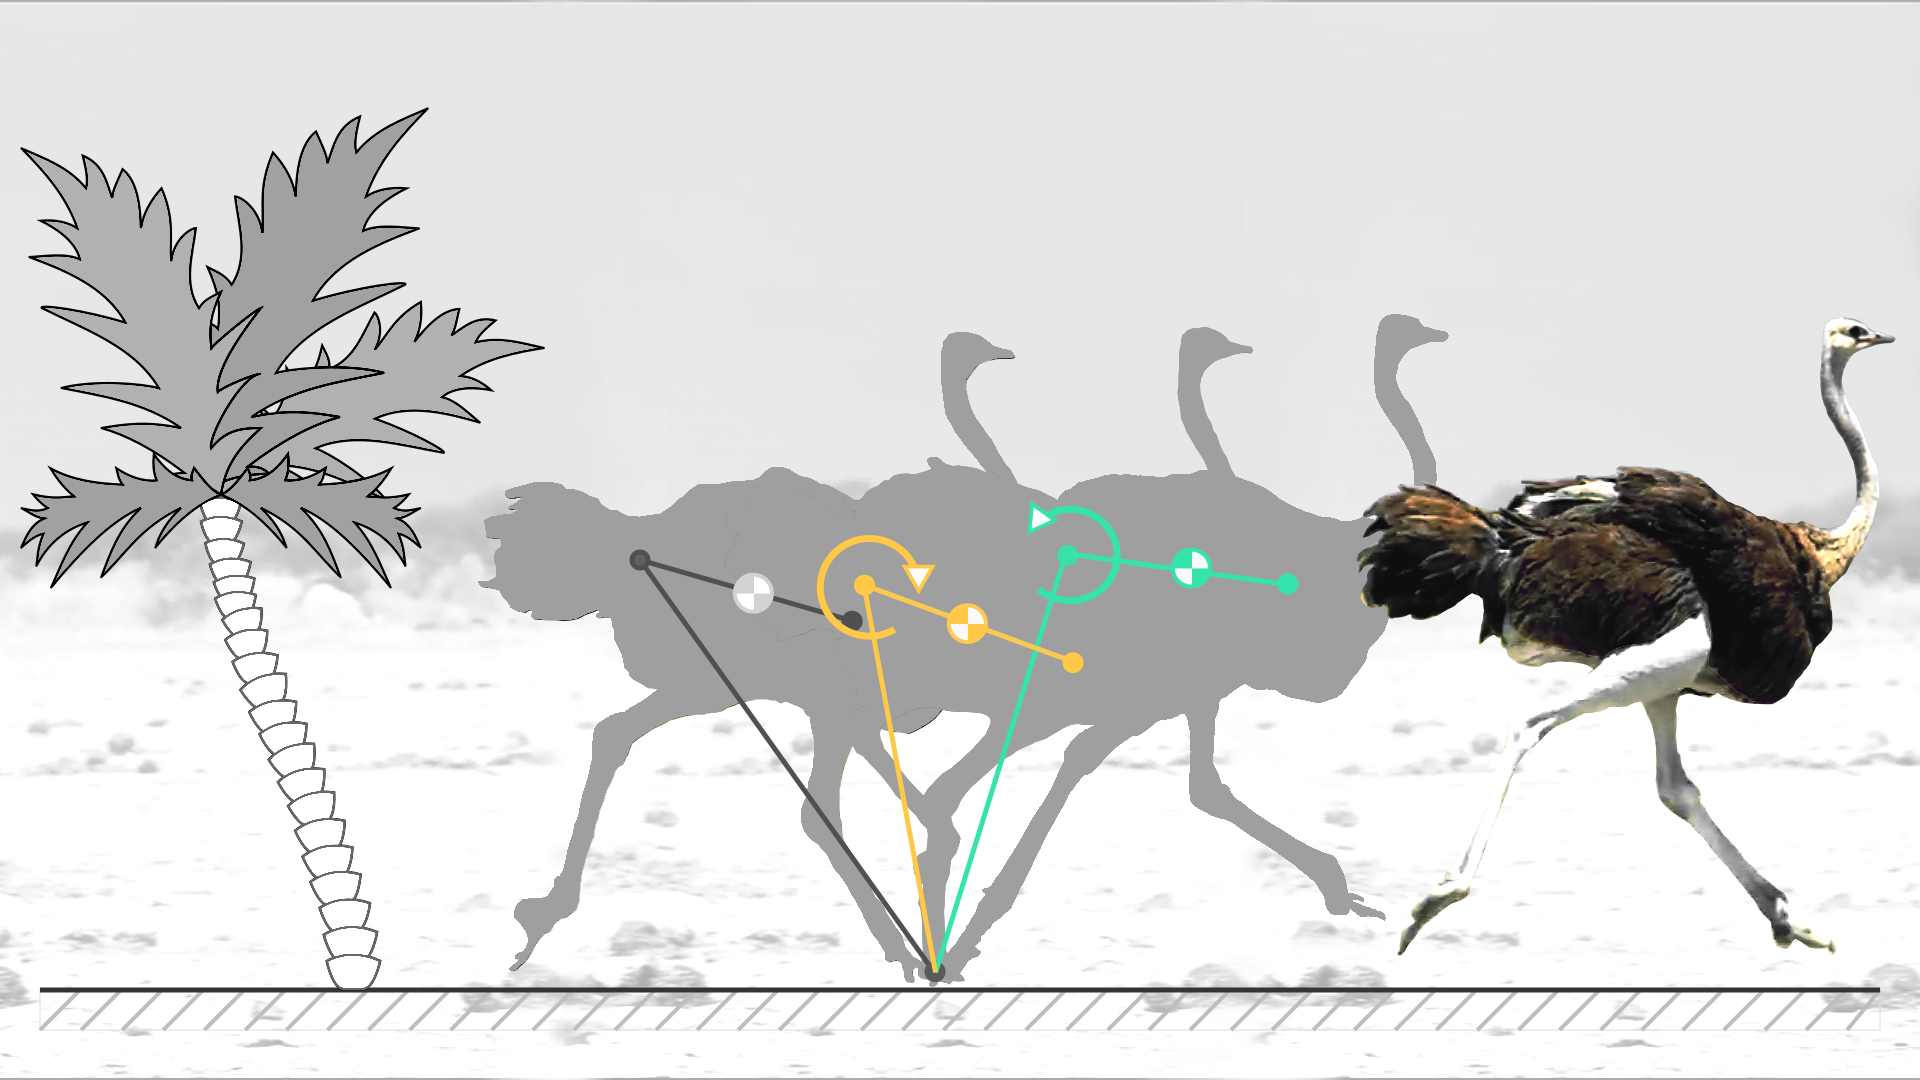
\includegraphics[scale=0.2]{figures/gaitostr.png}
% \caption{Gait of Ostrich - Walking}
% \label{fig:ostrgait}
% \end{figure*}

Inspired by these biomechanics principles, researchers have been developing bipedal robots capable of imitating the natural gaits. These robots use sophisticated control algorithms to replicate the alternating and synchronous gait patterns found in animals. Such designs enhance mobility, making them suitable for rescue missions or autonomous exploration applications. Researchers developed walking algorithms for different requirements of inclination and topography of the terrain and tested them in physics-based simulators and on the physical robot, which showed promising performance \cite{daley2019running} \cite{pratt2008design}.

\begin{figure*}[h!]
\centering
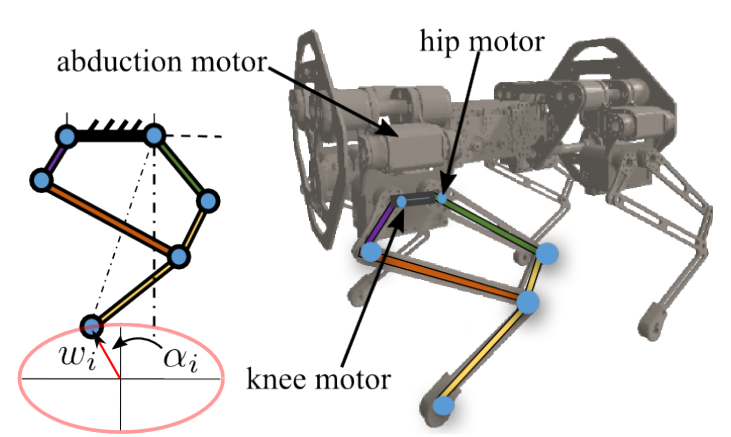
\includegraphics[scale=0.5]{figures/fivebar.png}
\caption{A five-bar mechanism is used as the legs of the quadruped robot. This mechanism is actuated by the motors located at the main torso of the robot \cite{tirumala2019gait}}
\label{fig:fivebar}
\end{figure*}

This project is based on the design explored in \cite{tirumala2019gait}, where rigid links were used to form a five-bar mechanism, as shown in Figure \ref{fig:fivebar}. Using reinforcement learning, libraries of walking trajectories were generated to deploy onto the physical robot; these libraries included different gaits, including trot, side-step, etc. While this robot is made using rigid links, our project focuses on leveraging the concept of using a foldable mechanism to form limbs of the biped using the five-bar mechanism; this offers greater adaptability and compliance, allowing it to absorb shocks and adjust dynamically to uneven terrain, unlike rigid-link designs that can transmit high-impact forces directly to joints. This flexibility enhances energy efficiency and stability, especially in complex environments, by mimicking the natural elasticity found in animal limbs.



%---------------------------------------------------------------------------------------------%

\section*{Goal Performance Metrics}

The primary objective of this research is to conduct a systematic analysis and characterization of gait patterns in quadruped robots, focusing on walking and galloping behaviors. The study aims to understand how specific morphological features, such as knee length and foot geometry, influence the robot's overall speed, stability, and energy efficiency performance. A comprehensive set of performance metrics has been defined to achieve this, encompassing kinematic, dynamic, and contact-based parameters. These metrics will be assessed through simulations using MuJoCo, with validation via precise tracking of link positions of the hardware prototype. The following sections elaborate on the specific goals and associated performance metrics.

\subsection*{1. Locomotion Performance}
\subsubsection*{1.1. Maximum Forward Walking Speed}
Maximum forward walking speed represents the highest achievable velocity during stable locomotion. In a 5-bar linkage mechanism, this is fundamentally limited by actuator capabilities, link lengths, and inertial properties \cite{zhou2020}.
The maximum achievable forward velocity is primarily determined by:
\begin{equation}
    v_{max} = f(P, l, \theta_{max}, m(x))
\end{equation}
where:
\begin{itemize}
    \item $P$ = actuator power output
    \item $l$ = characteristic leg length
    \item $\theta_{max}$ = joint range limits
    \item $m(x)$ = mass distribution function
\end{itemize}

\subsubsection*{1.2 Cost of Transport (CoT)}
CoT measures the energy efficiency of locomotion, which is particularly important for battery-powered robots. For 5-bar linkages, this metric is heavily influenced by the mechanical design and actuation strategy \cite{rezazadeh2018}. Energy efficiency metric defined as:
\begin{equation}
    \text{CoT} = \frac{E}{mgd}
\end{equation}
where:
\begin{itemize}
    \item $E$ = total energy consumed
    \item $m$ = robot mass
    \item $g$ = gravitational acceleration
    \item $d$ = distance traveled
\end{itemize}

\subsection*{2. Control System Performance}
\subsubsection*{2.1 Joint Position Accuracy}
Position accuracy determines the precision of foot placement and overall motion control. In 5-bar linkages, this is complicated by the coupled nature of the parallel mechanism \cite{kuindersma2016}.
Position error is defined as:
\begin{equation}
    \epsilon_{pos} = f(\text{sensor resolution}, \text{backlash}, \text{rigidity})
\end{equation}

\subsection*{3. Payload Performance}
\subsubsection*{3.1 Maximum Payload Capacity}
Payload capacity defines the maximum additional mass the robot can carry while maintaining stability and performance \cite{park2021}. This is particularly important for service robots or industrial applications.
Load carrying capability:
\begin{equation}
    m_{payload} = f(\tau_{max}, \text{structural strength})
\end{equation}
Subject to stability constraint:
\begin{equation}
    \text{CoM}_{total} \in \text{support polygon}
\end{equation}

\subsubsection*{3.2 Stability Impact}
Stability metrics ensure the robot maintains balance during locomotion and load carrying. The ZMP criterion is particularly important for dynamic stability \cite{vukobratovic2004}.
Payload-dependent stability metric:
\begin{equation}
    S_{payload} = f(A_{foot}, m(x), \text{CoM}_{height})
\end{equation}
where $A_{foot}$ represents foot contact area.

\noindent\hrulefill % Adds a horizontal line

\vspace{10pt} % Adds extra vertical space
These performance metrics and their impact on the design of the bipedal robot are described in Table \ref{tab:metrics}

\begin{table}[H]
\centering
\renewcommand{\arraystretch}{1.3} % Adjusts row height
\setlength{\tabcolsep}{10pt} % Adjusts column spacing
\scriptsize % Reduces the font size for the table
\resizebox{\textwidth}{!}{ % Scales the table to fit the page width
    \begin{tabularx}{\textwidth}{|X|X|}
    \hline
    \rowcolor{gray!20}
    \textbf{Performance Metric} & \textbf{Design Constraints} \\
    \hline
    \multicolumn{2}{|l|}{\cellcolor{gray!10}\textbf{1. Locomotion Performance}} \\
    \hline
    Maximum Forward Walking Speed & 
    \begin{itemize}
        \item Actuator torque-speed characteristics
        \item Link length ratios ($L_1/L_2$, $L_3/L_4$)
        \item Maximum joint angular velocities
        \item Mechanical transmission limits
    \end{itemize} \\
    \hline
    Cost of Transport (CoT) & 
    \begin{itemize}
        \item Motor efficiency curves
        \item Transmission efficiency
        \item Link mass distribution
        \item Joint friction characteristics
    \end{itemize} \\
    \hline
    \multicolumn{2}{|l|}{\cellcolor{gray!10}\textbf{2. Control System Performance}} \\
    \hline
    Joint Position Accuracy & 
    \begin{itemize}
        \item Encoder resolution
        \item Mechanical backlash
        \item Link/joint stiffness
        \item Controller bandwidth
    \end{itemize} \\
    \hline
    \multicolumn{2}{|l|}{\cellcolor{gray!10}\textbf{3. Payload Performance}} \\
    \hline
    Maximum Payload Capacity & 
    \begin{itemize}
        \item Maximum actuator torque
        \item Structural strength of links
        \item Joint bearing load ratings
        \item Static/dynamic stability margins
    \end{itemize} \\
    \hline
    Stability Impact & 
    \begin{itemize}
        \item Foot contact area
        \item Center of mass location
        \item Ground reaction force limits
        \item ZMP constraints
    \end{itemize} \\
    \hline
    \end{tabularx}
}
\caption{Performance Metrics and Design Constraints for 5-Bar Linkage Bipedal Robot}
\label{tab:metrics}
\end{table}


% \begin{table}[H]
% \centering
% \renewcommand{\arraystretch}{1.3} % Adjusts row height
% \setlength{\tabcolsep}{10pt} % Adjusts column spacing
% \begin{tabularx}{\textwidth}{|X|X|}
% \hline
% \rowcolor{gray!20} % Corrected color definition
% \textbf{Performance Metric} & \textbf{Design Constraints} \\
% \hline
% \multicolumn{2}{|l|}{\cellcolor{gray!10}\textbf{1. Locomotion Performance}} \\
% \hline
% Maximum Forward Walking Speed & 
% \begin{itemize}
%     \item Actuator torque-speed characteristics
%     \item Link length ratios ($L_1/L_2$, $L_3/L_4$)
%     \item Maximum joint angular velocities
%     \item Mechanical transmission limits
% \end{itemize} \\
% \hline
% Cost of Transport (CoT) & 
% \begin{itemize}
%     \item Motor efficiency curves
%     \item Transmission efficiency
%     \item Link mass distribution
%     \item Joint friction characteristics
% \end{itemize} \\
% \hline
% \multicolumn{2}{|l|}{\cellcolor{gray!10}\textbf{2. Control System Performance}} \\
% \hline
% Joint Position Accuracy & 
% \begin{itemize}
%     \item Encoder resolution
%     \item Mechanical backlash
%     \item Link/joint stiffness
%     \item Controller bandwidth
% \end{itemize} \\
% \hline
% \multicolumn{2}{|l|}{\cellcolor{gray!10}\textbf{3. Payload Performance}} \\
% \hline
% Maximum Payload Capacity & 
% \begin{itemize}
%     \item Maximum actuator torque
%     \item Structural strength of links
%     \item Joint bearing load ratings
%     \item Static/dynamic stability margins
% \end{itemize} \\
% \hline
% Stability Impact & 
% \begin{itemize}
%     \item Foot contact area
%     \item Center of mass location
%     \item Ground reaction force limits
%     \item ZMP constraints
% \end{itemize} \\
% \hline
% \end{tabularx}
% \caption{Performance Metrics and Design Constraints for 5-Bar Linkage Bipedal Robot}
% \label{tab:metrics}
% \end{table}



%---------------------------------------------------------------------------------------------%

\section*{Specifications Table}

\begin{table}[H]
\centering
\renewcommand{\arraystretch}{1.3}
\begin{tabular}{p{0.35\textwidth} p{0.1\textwidth} l p{0.2\textwidth}}
\toprule
\textbf{Parameter} & \textbf{Value} & \textbf{Unit} & \textbf{Reference} \\
\midrule
\multicolumn{4}{l}{\textit{Locomotion Performance}} \\
Maximum Walking Speed & 1.5 & \si{m/s} & \cite{zhou2020} \\
Cost of Transport & 0.2 & dimensionless & \cite{rezazadeh2018} \\
Link Length Ratio ($L_1/L_2$) & 1.2 & dimensionless & \cite{liu2021} \\
\midrule
\multicolumn{4}{l}{\textit{Control System}} \\
Joint Position Accuracy & 0.01 & \si{rad} & \cite{kuindersma2016} \\
\midrule
\multicolumn{4}{l}{\textit{Payload Performance}} \\
Maximum Payload & 0.1 & \si{kg} & \cite{park2021} \\
Maximum Actuator Torque & 0.1765 & \si{N.m} & Design spec \\
Link Mass (per leg) & 0.05 & \si{kg} & Design spec \\
Foot Contact Area & 0.002 & \si{m^2} & Design spec \\
Ground Clearance & 0.05 & \si{m} & Design spec \\
\bottomrule
\end{tabular}
\caption{Specifications Table for 5-Bar Linkage Bipedal Robot}
\label{tab:specifications}
\end{table}




%---------------------------------------------------------------------------------------------%

\section*{Develop an analogous mechanism }
% Develop an analogous mechanism for your source of bio-inspiration in paper or cardboard.
The diagram illustrates a bipedal gait bio-mimicry system's left and right leg mechanisms. Being a 5 bar linkage mechanism, each leg consists of interconnected joints and links (labeled \( l_1, l_2, \ldots, l_5 \)) with various points of rotation (\( P_{0}, P_{1}, P_{2},P_{00}, P_{11}, P_{22}, \) etc.)  and orientation vectors. These components are organized to simulate natural gait dynamics, with angles (\( \Theta_1, \Theta_2, \ldots \)) representing joint movements. The foldable aspect allows the leg to compactly retract, contributing to efficient energy usage and realistic movement.

The mechanism operates under specific angle constraints that are critical for achieving realistic and efficient motion. Each joint angle, denoted as \( \Theta_1, \Theta_2, \Theta_3, \Theta_4 \), is constrained within a predefined range to mimic the natural motion of bird legs. These constraints ensure that the legs move within permissible limits to prevent excessive bending, thereby maintaining the stability and balance of the mechanism during gait cycles.

These angle constraints are optimized to synchronize the movement of both the left and right legs, allowing for an alternating pattern that promotes a balanced, efficient, and bird-like gait. Moreover, the constraints also help in energy conservation by preventing excessive movements, enhancing the mechanism's overall efficiency.

\begin{figure}[H]
    \centering
    \subfigure[]{
        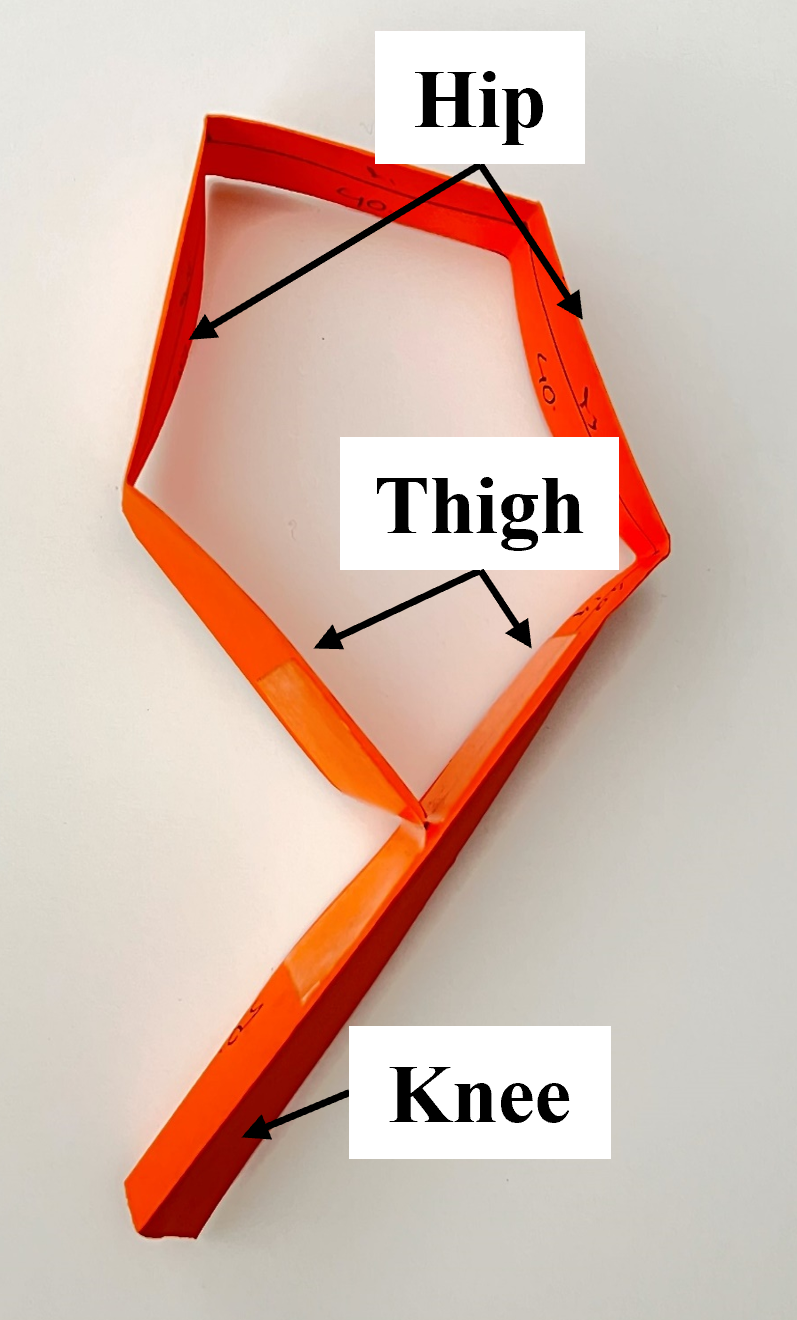
\includegraphics[scale = 0.5]{figures/Picture1.png}
    }
    \subfigure[]{
        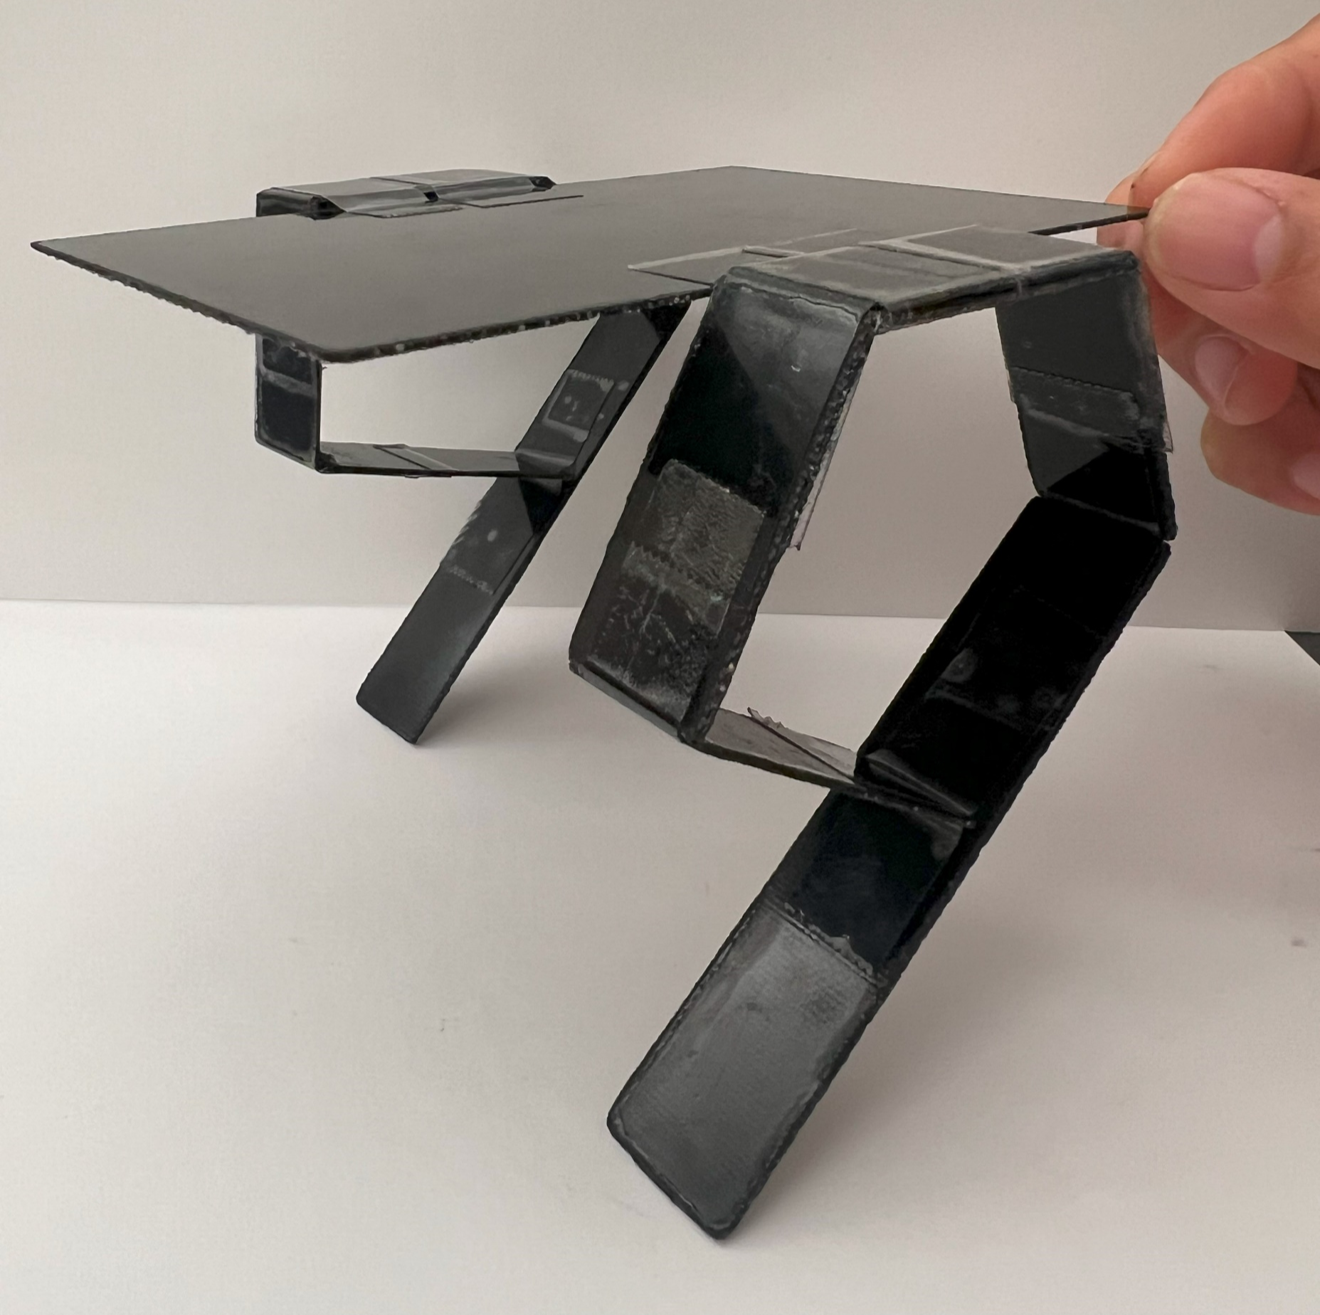
\includegraphics[scale = 0.5]{figures/Picture2.png}
    }
    \subfigure[]{
        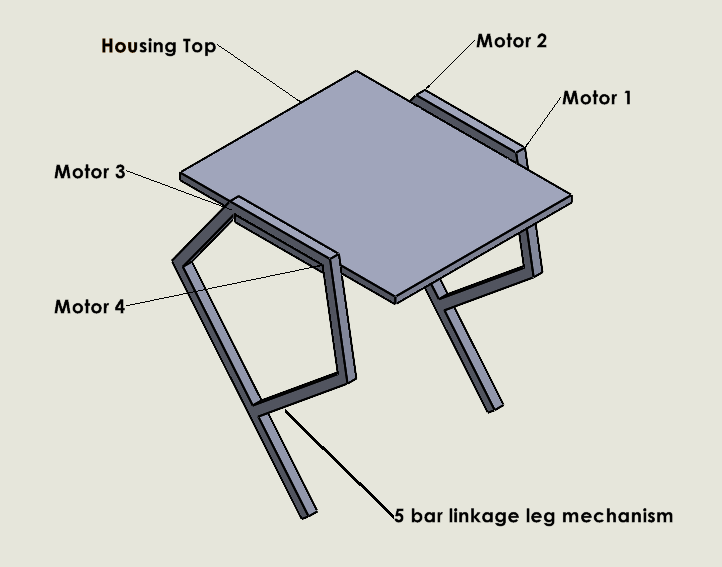
\includegraphics[scale = 0.5]{figures/Mechanism.png}
    }
    \caption{Proposed hardware prototype model of the bipedal robot; (a) A paper-based model ; (b) Hardware Model made from Fiberglass Sheet (c) CAD Representation of the Bipedal Robot .}
    \label{fig: proposed_prototype}
\end{figure}

% \begin{enumerate}
%     \item \textbf{Make the mechanism.} It can be cut by hand, but must clearly communicate where motor(s) will be connected, what touches the ground, and be able to move through its proposed range of motion from (only) motion about the actuators. Take pictures of it in multiple configurations of its gait cycle.
%     \begin{itemize}
%         \item The mechanism should use a link / joint topology and the folding approach for making joints that you have learned from this class.
%         \item Consider using parallel and series mechanisms as they are best suited.
%         \item Consider both planar and spherical mechanisms as appropriate for your needs.
%         \item Consider where to eventually place springs.
%     \end{itemize}
    

    \begin{figure}[H]
    \centering
    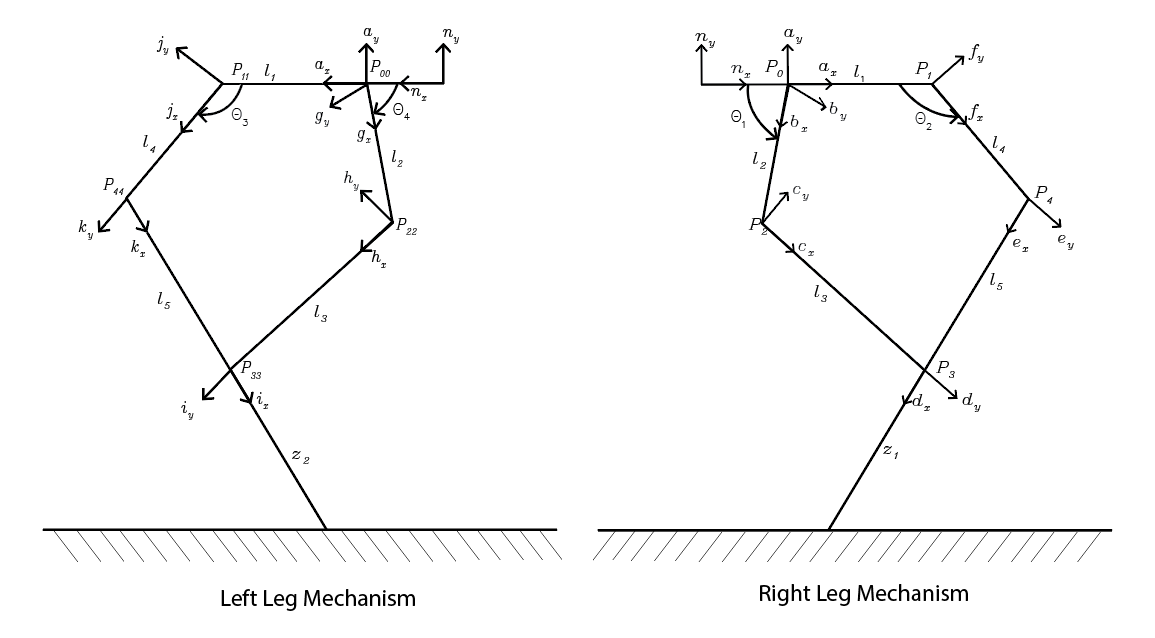
\includegraphics[scale=0.5]{figures/vecdiagram.png}
    \caption{Vector Drawing}
    \label{fig:mechanism}
    \end{figure}
    
    
%     Use a vector drawing program (Inkscape, IPE, Illustrator, Draw.io) or 3D modeling software to ensure a professional result.
%     \begin{itemize}
%         \item Label each reference frame, including your inertial (Newtonian) reference frame.
%         \item Include a set of orthonormal basis vectors for each frame ($\hat{n}_x, \hat{n}_y, \hat{n}_z$), ($\hat{a}_x, \hat{a}_y, \hat{a}_z$). It is best practice to align one of the basis vectors (like $\hat{a}_x$) with each rigid link.
%         \item Variable names for each state variable ($\theta_1, \theta_2, \dot{\theta}_1, \dot{\theta}_2, ...$)
%         \item Geometric values such as link lengths ($l_1, l_2, ...$)
%     \end{itemize}
    
%     \begin{center}
%         \fbox{\begin{minipage}{0.9\textwidth}
%         \textbf{Save this figure for reuse later.} You will need to add mass and inertial information as well as system stiffness information, so make sure you do your work in a way that permits reusing and modifying the figure.
%         \end{minipage}}
%     \end{center}
% \end{enumerate}




%---------------------------------------------------------------------------------------------%

\section*{System Identification}


\subsection*{1. Actuator Parameters}
\begin{itemize}
    \item Motor resistance: measured directly with a multimeter
    \item Motor inductance: measured with RLC meter
    \item Rotor inertia: derived from step response
    \item Gear ratio efficiency: from the input-output power measurement
\end{itemize}

\subsection*{2. Mass and Inertia Properties}
\begin{itemize}
    \item Link masses: direct measurement of fabricated parts
    \item Center of mass locations: balancing test for each link
    \item Combined leg inertia: using swing test of assembled leg
\end{itemize}

\subsection*{3. Stiffness and Damping Characteristics}
\begin{itemize}
    \item Joint stiffness: force-deflection measurements
    \item Link structural stiffness: static loading test
    \item Link material damping: impact response test
\end{itemize}


\subsection*{4. Experimental Methods}

\subsubsection*{4.1 Motor Characterization}
\begin{itemize}
    \item Setup: Motor test bench with torque sensor and encoder
    \item Measurements: Current, voltage, position, velocity
    \item Equipment: Power supply, DAQ, oscilloscope
\end{itemize}

\subsubsection*{4.2. Link Properties}
\begin{itemize}
    \item Setup: Precision scale, pendulum test rig
    \item Measurements: Mass, period of oscillation
    \item Equipment: High-speed camera
\end{itemize}

\subsubsection*{4.3. Simulation Verification}
\begin{itemize}
    \item Setup: Gait testing on hardware
    \item Measurements: Mass, walking speed, joint trajectory
    \item Equipment: MuJoCo
\end{itemize}

\subsubsection*{4.4. Model Verification}
\begin{itemize}
    \item Setup: Gait testing on hardware
    \item Measurements: Mass, walking speed, joint trajectory
    \item Equipment: High-speed camera, markerless-tracking software
\end{itemize}

\begin{table}[htbp]
\centering
\renewcommand{\arraystretch}{1.3}
\begin{tabular}{|p{0.4\textwidth}|c|c|c|}
\hline
\textbf{Experiment} & \textbf{Jahnav} & \textbf{Kunal} & \textbf{Nihar} \\
\hline
Motor Characterization \& System Integration & X & & \\
\hline
Link Stiffness \& Simulation Verification & & X & \\
\hline
Hardware Verification \& Simulation Comparision & & & X \\
\hline
\end{tabular}
\caption{System Identification Experiments and Team Assignment}
\label{tab:experiments}
\end{table}


% The purpose of this part is to create a plan for identifying key model parameters that teammates will be able to execute individually, and then contribute back to their team’s modeling effort. This should include aspects from the following:

% %\textbf{Just elaborate more in this} 

% \begin{itemize}
%     \item Actuator parameters – resistance, inductance, inertia, damping, mass, $K_v / K_\tau$, gearing – fit against experimental data.
%     \item The mass and inertia properties of key parts of your proposed system, modeled and verified.
%     \item The stiffness and damping characteristics:
%     \begin{itemize}
%         \item of your team’s joints, as fabricated.
%         \item of your team’s links, as fabricated.
%         \item of a key subsystem, as fabricated.
%         \item of a discrete energy storage component.
%     \end{itemize}
%     \item Friction estimations and a model fitting process between key materials undergoing contact interactions.
%     \item ...other ideas approved by your professor.
% \end{itemize}

% \begin{enumerate}
%     \item Identify and discuss the various parameters you plan to model in your simulation. Discuss your plans for experimentally obtaining each of those values, and the model you would like to use for describing each phenomenon.
    
%     \item Create a table with at least four system identification experiments you will run, and an assigned team lead for each experiment.
% \end{enumerate}

% \begin{table}[h]
% \centering
% \begin{tabular}{|l|c|c|c|}
% \hline
% \textbf{Item} & \textbf{Jahnav} & \textbf{Kunal} & \textbf{Nihar} \\
% \hline
% Servo Characterization and Synchronization & x &  &  \\
% Link Stiffness Experiment &  & x &   \\
% Joint Stiffness Experiment &  &  & x  \\
% \hline
% \end{tabular}
% \caption{System Identification Experiments and Assigned Team Leads}
% \end{table}

% \noindent Individual experiments will be assigned to each team member as part of an upcoming individual assignment.



%---------------------------------------------------------------------------------------------%

\section*{Project Part 2 Roadmap}

This project requires multi-level planning and execution, which includes a material selection for joints and links, estimates for approximate lengths, prototyping multiple iterations of joint mechanisms, kinematic analysis, simulation using MuJoCo, implementing servo motors, and controlling the robot using microcontroller, collecting data for further analysis. The project roadmap is as follows:

Materials: Legs hold the weight of the robot and all its components while giving mobility, the structural rigidity of the links and joint play a crucial role. Fiberglass is a structurally rigid material which is still flexible to give a natural compliance to the leg, a very thin (0.5 mm) fiber glass sheet is used to make links while a plastic adhesive tape is used to connect the links and form a joint as shown in previous section. Servo motors will be housed on the top of robot using a 3D printed housing that can hold the motor in place, micro controller and power supply are to be placed off board to minimize the load on the legs for the robot.

One person from the team takes care of prototyping multiple iterations of the robot with different joint parameters until the optimized design is achieved. The body will be kept modular to accommodate multiple iterations of legs with varying parameters and end effector geometries, which is crucial to maintaining enough contact with the ground to leverage friction and move forward or backward.

System data can be analyzed by tracking the motion of the joints, this can be done by taking a video of the joints moving with a given input signal to the servo motors and then further using a Tracker software to plot the mechanism while performing multiple gaits. This can further be validated by simulating the same mechanism in MuJoCo. The performance metrics as specified above (stride length, stride frequency, linear speed and trajectory tracking) can be analyzed using the robot's position tracked from the video. These data points can be visualized using either MATLAB or Python.

Simulation can be done in multiple parts, which include writing the code to define the model and set up the robot, defining the parameters and setting up the experiments, data collection, and model fitting and validating with the experimental data. One of the team mates focuses on writing the code while the others focus on the protocol and parameters of the study, data analysis is planned to be done by everyone post collection to keep everyone in the loop about the final results.

The collected data can be used to make plots that show statistical significance over different gaits and experimental studies; all of these plots and relevant images can be used to make a detailed report along with a folder that contains the simulation and data processing codes and files, all of these can be submitted the end of the semester.



% Finally, plan the upcoming tasks and roles for the other team activities. Write up your plan for the following:
% \begin{enumerate}
%     \item Identify and discuss the materials you plan to use in fabrication, and key design decisions, such as how you plan to fabricate parts. Decide who will be obtaining those materials and distributing them.
    
%     \item Identify and discuss how you plan to prototype your system and assign one person to do that.
    
%     \item Identify and discuss how you will collect system-level motion or force data for validation, including:
%     \begin{itemize}
%         \item method (IMU, video, discrete joint sensors, force/torque sensing)
%         \item data extraction approach
%         \item how you plan to characterize performance. What metrics will you use and what experiments do you need to measure that performance?
%         \item how you plan to visualize your data.
%     \end{itemize}
    
%     \begin{center}
%         \fbox{\begin{minipage}{0.9\textwidth}
%         \textbf{Note:} We are distinguishing from component level model fitting, which should come before you add elements to your model, and verification / validation experiments, which should come after you have built your final device.
%         \end{minipage}}
%     \end{center}
    
%     \item Identify and discuss your plan for shared simulation tasks:
%     \begin{itemize}
%         \item who will be working with the code
%         \item adding model fitting routines
%         \item filtering, interpolating, and otherwise massaging input data
%         \item optimization approach
%     \end{itemize}
    
%     \item Identify and discuss any reporting tasks that may be needed:
%     \begin{itemize}
%         \item compiling information into a report (may be combined with the simulation if using Jupyter)
%         \item managing the GIT repository
%     \end{itemize}
    
%     \item Split each of these tasks to the individuals on your team and visualize task assignments in a table.
% \end{enumerate}



% \begin{itemize}
%     \item Project Definition - Jahnav, Nihar
%     \item Background Research - Jahnav
%     \item Initial Calculations - Kunal, Jahnav
%     \item Specifications Table - Nihar
%     \item Modeling and Analysis - Kunal, Nihar
%     \item Mechanism Prototype and Figure - Jahnav, Kunal
%     \item System Identification Plan and Roadmap - Jahnav, Kunal, Nihar
% \end{itemize}

%---------------------------------------------------------------------------------------------%
% Add bibliography here
\bibliographystyle{IEEEtran}
\bibliography{references}

\end{document}